\documentclass[11 pt, twocolumn]{article}

\usepackage{hyperref}
\usepackage{titling}
\usepackage{amsmath}
\usepackage{algorithm}
\usepackage[noend]{algpseudocode}
\usepackage[margin=0.8in]{geometry}
\usepackage{graphicx}
\usepackage{color}

\makeatletter
\def\BState{\State\hskip-\ALG@thistlm}
\makeatother

\setlength{\droptitle}{-5em}
\setlength{\columnsep}{2em}
 
\title{Novel Ideas For ES}
\author{Nevo Agmon 203116769, Yuval Shildan 205799307}
\date{Winter 2019}

\newcommand{\todo}[1]{{\color{red} TODO: {#1}}}
\newcommand{\algspace}{\hspace{\algorithmicindent}}

\begin{document}
\maketitle
\section{Abstract}
In the field of AI Reinforcement Learning (RL) is used to solve problems requiring an agent to interact with a given environment. Specifically, Q - Learning is a model free algorithm with the goal of learning a policy which tells the agent what action to take in a given state.

Evolution Strategies (ES) is a family of algorithms based on the idea of natural evolution that have recently shown to be comparable to the state of the art in Q - Learning on a challenging set of problems. ES have the benefit of being highly parallelizable, thus reducing training duration from several days to a matter of hours.

ES and RL have different learning characteristics, resulting in different strengths and weaknesses. In this paper we describe a very simple canonical ES algorithm, and try to improve it's performance with ideas from more traditional RL in order to show that the combination of both could possibly advance upon the current state of the art.


\section{Problem Description}
Our work is based on the paper \emph{Back to Basics: Benchmarking Canonical Evolution Strategies for  Playing Atari}, by Chrabaszcz et al. \cite{canonical} in which a canonical ES algorithm is described and benchmarked on a series of Atari games. The algorithm is described in Algorithm \ref{alg:canonical}.

\subsection{CanonicalES}
As can be seen the algorithm is based on an iterative process where in every iteration $t$ we create a set of $\lambda$ offspring. This is done by adding a mutation to the base policy, the mutation is given by the mutation step size multiplied by a sampled random noise. After offspring creation we evaluate each offspring's policy on the environment. Once this process in done, we choose the $\mu$ best performing offspring and update the base policy with the weighted sum of their mutation.

This algorithm is relatively simple, and as mentioned before, is loosely based on the idea of natural evolution. Meaning, offspring are passed the "genetic material" from their parent with a random mutation, evolution occurs when processes like natural selection acts on these variations and results in some characteristics being more prominent in the population while others become sparse.

\begin{algorithm}
\scriptsize
\caption{CanonicalES Algorithm}\label{alg:canonical}
\hspace*{\algorithmicindent} \textbf{Input:} \\
\hspace*{\algorithmicindent} $\sigma$ - Mutation step size\\
\hspace*{\algorithmicindent} $\theta_0$ - Initial Policy parameters\\
\hspace*{\algorithmicindent} $F$ - Policy evaluation function\\
\hspace*{\algorithmicindent} $\lambda$ - Offspring population size\\
\hspace*{\algorithmicindent} $\mu$ - Parent population size\\
\hspace*{\algorithmicindent} \textbf{Initialize:}
\begin{align*}
  &w_i=\frac{\log{(\mu + 0.5)}-\log{(i)}}{\sum_{j=1}^{\mu} \log{(\mu + 0.5)}-\log{(j)}}&
\end{align*}
\begin{algorithmic}[1]
      \For{$t \in \{0,1,\dots\}$}
      	\For{$i \in \{1,\dots,\lambda\}$}
      	\State Sample noise: $\epsilon_i \sim \mathcal{N}(0,I)$
      	\State Evaluate score in the game: $s_i \gets F(\theta_t+\sigma*\epsilon_i)$
      	\EndFor
      	\State Sort($\epsilon_1,\dots,\epsilon_\lambda$) according to $s$ ($\epsilon_i$ with best $s_i$ first)
      	\State Update policy: $\theta_{t+1} \gets \theta_t + \sigma * \sum_{j=1}^{\mu} w_j*\epsilon_j$
      	\State Optionally update step size $\sigma$
      \EndFor
\end{algorithmic}
\end{algorithm}

\subsection{Main Objective}
This approach yielded good results in a short period of training, as shown by Chrabaszcz et al. but has few drawbacks, as shown in figure \ref{fig:canonical_results}. The main drawbacks are that the policy tends to reach some local optima and plateaus. This leads to the main objective of this paper, define a set of improvements to encourage the policy to seek for a better solution and reduce the tendency to plateau. To accomplish this objective we look at the work done by Conti et al. \cite{improveES} in the paper \emph{Improving Exploration in Evolution Strategies for Deep Reinforcement Learning via a Population of Novelty-Seeking Agents}. In their paper Conti et al. try to optimize an ES algorithm (related but not the same as Chrabaszcz et al.'s canonical one) for seeking novel decisions to address the very same problem.

\begin{figure}[h!]
  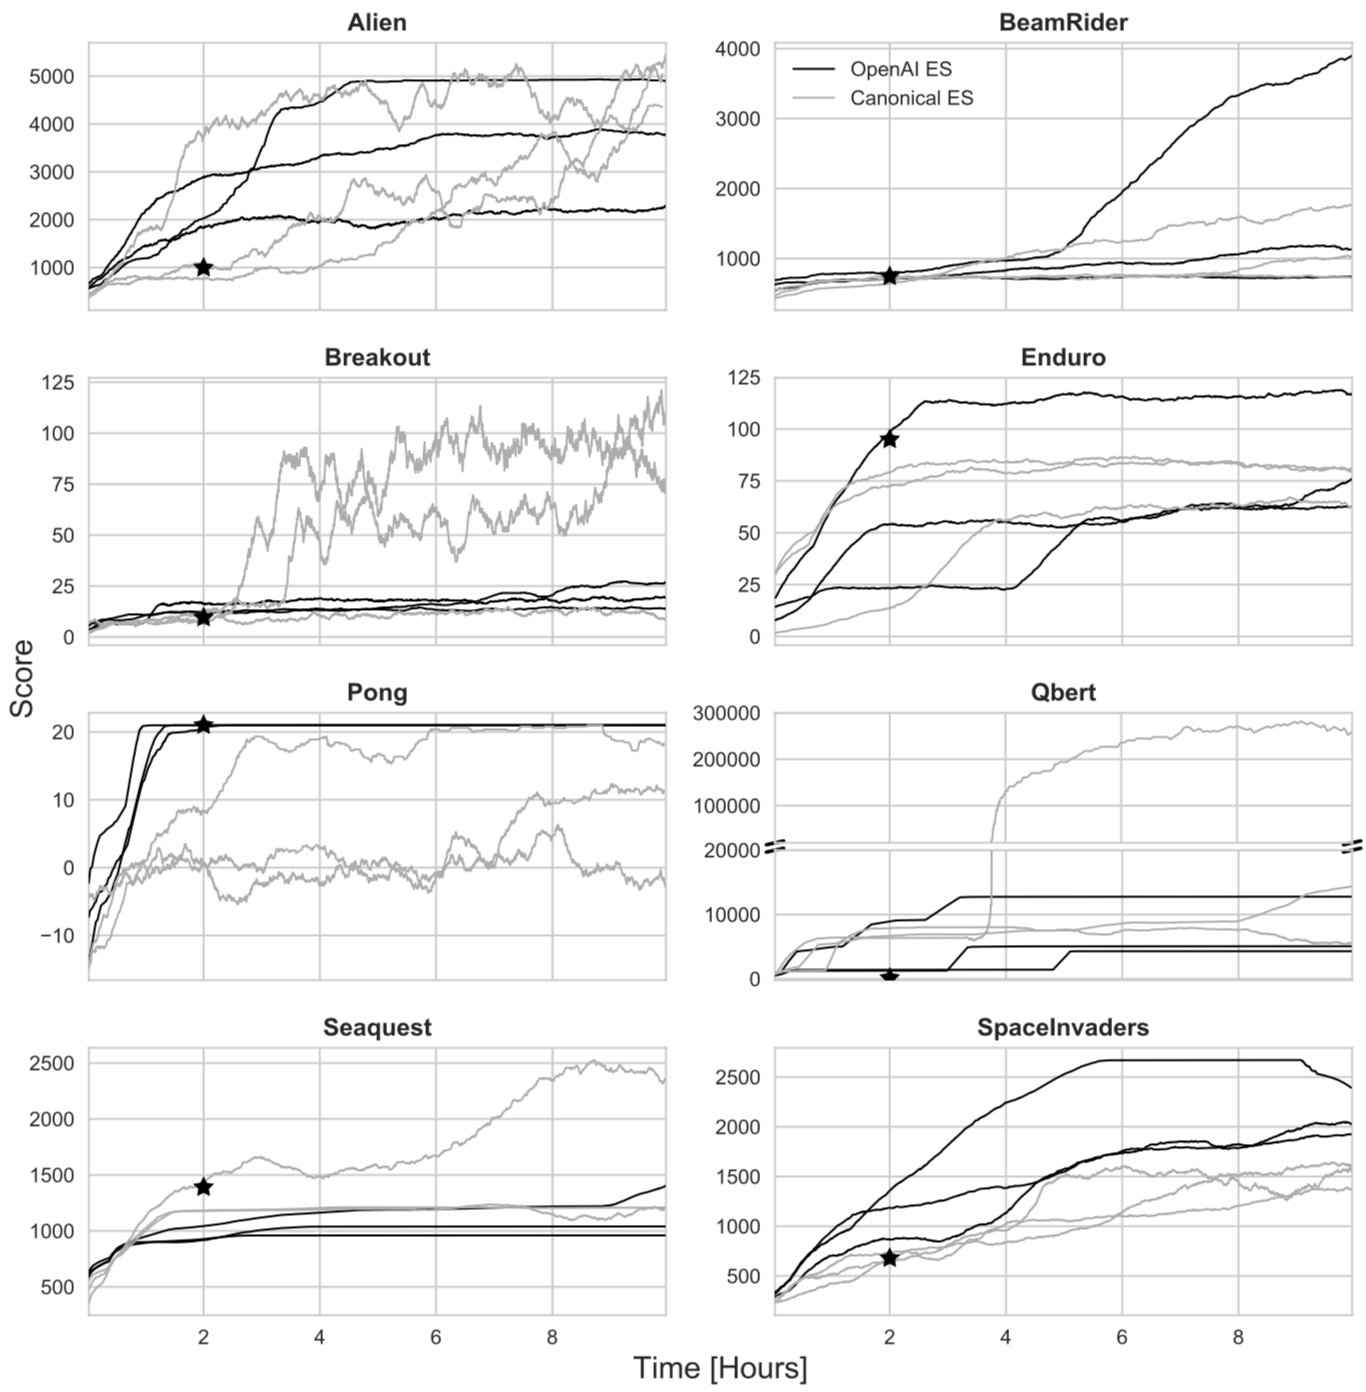
\includegraphics[width=\linewidth]{canonical_train_res.png}
  \caption{Training curves for Chrabaszcz et al.'s CanonicalES algorithm. The algorithm often reach local optima and plateaus.}
  \label{fig:canonical_results}
\end{figure}

\section{Method Description}
To define a set of improvements to try and rectify the described problem we first had to make an assumption as to what causes this behavior. Our assumption was that because the algorithm optimizes for immediate reward, it can miss on the opportunity for better performance and greater overall reward. Meaning, we want to optimize for overall game performance, preferably averaging performance over multiple runs. Unfortunately, since a single game is comprised of a large number of decisions, if we track the end game result and optimize accordingly we could not tell what is the state and action relations that improve performance and therefore optimize poorly.

Therefore, we decided to focus on two aspects of the algorithm for improvement:
\begin{enumerate}
	\item Searching for new untried moves.
	\item Reproduce population from multiple samples.
\end{enumerate}

\subsection{Novelty Search}\label{sec:novelty}
In order to reduce the tendency to reach local optima biased by short term reward we introduce Novelty Search (NS). As shown by Conti et al. NS encourages the policy to act differently than previous seen behavior. To encourage different behaviors the algorithm uses a \emph{novelty} value computed for each policy to represent the amount of innovation of the current policy with respect to the previously seen policies.

Formally, given a parameter vector $\theta$  and policy $\pi_\theta$ we define a \emph{behavior} mapping $b(\pi_\theta)$, this can be thought of as an embedding of the policy output to a vectorized form. We then save these behavior representations in a set $A$ and evaluate the \emph{novelty} of the current policy as the average distance between it and the $k$ nearest neighbors from the saved set $A$.

\begin{align*}
N(\theta, A)=N(b(\pi_\theta),A)&=\frac{1}{|S|}\sum_{j\in S} \|b(\pi_\theta)-b(\pi_j)\|_2\\
S=kNN(b(\pi_\theta),A)&=\{b(\pi_1),b(\pi_2), \dots,b(\pi_k)\}
\end{align*}

Now, instead of choosing the meta population based on the policy's reward we want to take into account both the reward and policy's novelty. We assign each policy a performance score $\hat{s}$, it's novelty value added to it's reward:

\begin{equation*}
\hat{s}=N(\pi_\theta,A)+F(\theta)
\end{equation*}

To update the policy we can add the reward and novelty values to the update step thus encouraging the policy to move in the direction where the gradients of novelty and reward are greater. as a first try we add the novelty and reward average:

\begin{equation*}
\theta_{t+1}\gets\theta_t+\sigma*\sum_{j=1}^{\mu}w_j*\epsilon_j*\frac{N(\theta_t^j,A)+F(\theta_t^j)}{2}
\end{equation*}

To further improve our optimization we can weight the novelty and reward values according to the state we are in, as opposed to always having their average.

\begin{equation*}
\theta_{t+1}\gets\theta_t+\sigma*\sum_{j=1}^{\mu}w_j*\epsilon_j*(1-\hat{w})N(\theta_t^j,A)+\hat{w}F(\theta_t^j)
\end{equation*}

Starting with only optimization for reward ($\hat{w}=1$), we can track the policy's performance, if we improve our game we want to optimize for reward so in every iteration we increase the weight. If on the other hand we stop improving, it means we got into a plateau, we will start decreasing the weight so that we will optimize for novelty.

\subsection{Population Reproduction}
The CanincalES algorithm, as described, takes a meta population of size $\mu$ of best performing offspring and uses the weighted sum of their mutation as the learned parameter, updating the base policy with that weighted mutation. This may seem like a good idea: take the best of the population and reproduce them. But, if we take natural evolution as our guide for building our algorithm, then we know that the fact a beneficial mutation occurred is not directly correlated the offspring's ability to reproduce. Rather it simply increases the odes for the offspring reproduction and keep the mutation in the population. Therefore, instead of taking the best set of offspring we give each offspring a probability score based on it's performance and sample the set from the population according to the said probability.

We would like to use the performance score $\hat{s}$ we defined above to compute the probability, but depending on the domain the novelty and reward values may be at different scales. So we normalize these values. Given a population of size $\lambda$ the normalized novelty $\hat{N}$ and normalized reward $\hat{F}$ are defined as follows:

\begin{align*}
&\hat{N}(\theta,A)=\frac{N(\theta,A)}{\max_{\theta_i\in\{\theta_1,\theta_2,\dots,\theta_\lambda\}}N(\theta_i,A)}\\
&\hat{F}(\theta)=\frac{F(\theta)}{\max_{\theta_i\in\{\theta_1,\theta_2,\dots,\theta_\lambda\}}F(\theta_i)}
\end{align*}

Lastly, we define a probability value for each offspring. An offspring probability is defined as:

\begin{equation*}
P(\theta)=\frac{\hat{N}(\theta,A)+\hat{F}(\theta)}{\sum_{i=1}^{\lambda}\hat{N}(\theta_i,A)+\hat{F}(\theta_i)}
\end{equation*}

\subsection{Implementation}
As described in \ref{sec:novelty} we want to keep a set of behavior representation $A$ in order to compute the novelty score of an agent. The best scenario is to keep the state of the environment and the decision the player made, this is proven impossible due to memory restrictions. Keeping the state of the environment for every state would exceed the size of our memory very fast and want help us in computing the novelty score. In Conti et al.'s  paper the authors used a metric called RAM which is a vector of length 128 in the range [0,255]. The authors mentioned that this is only taken as a "proof of concept" and that a better representation is needed. We considered several options to solve this problem:
\paragraph{Deep Compression}
Our first approach was using deep compression, the idea is that compression of similar objects to ones the compressor has previously seen will be better (the output will be smaller) since the compressor learns to compress the objects. Thus novel decisions will lead to environment observations that the compressor has not seen before and will result in poor compression. The problem was that this approach is not yet polished enough to use in general problems and we had difficulty porting the implementations we found to our needs.
\paragraph{Auto-Encoder}
auto-encoder can be used to save the environment observation as the latent space representation which can be significantly smaller then it's original size. The problem was that we didn't had enough resources to run auto-encoder training while running the ES model training. Using more computation resource this can be a very good approach to consider.
\paragraph{PCA and KNN}
We finally decided to use PCA to reduce dimensionality of the data and then use KNN to find the nearest neighbors to the current policy from the PCA representation. In each iteration we took the $k$ nearest neighbors and calculated the sum of distances, higher distance means more novel solution.


Our final algorithm can be sen in Algorithm \ref{alg:our}.

\begin{algorithm}
\scriptsize
\caption{OurES Algorithm}\label{alg:our}
\hspace*{\algorithmicindent} \textbf{Input:} \\
\hspace*{\algorithmicindent} $\sigma$ - Mutation step size\\
\hspace*{\algorithmicindent} $\theta_0$ - Initial Policy parameters\\
\hspace*{\algorithmicindent} $F$ - Policy evaluation function\\
\hspace*{\algorithmicindent} $\lambda$ - Offspring population size\\
\hspace*{\algorithmicindent} $\mu$ - Parent population size\\
\hspace*{\algorithmicindent} \textbf{Initialize:}
\begin{align*}
  &w_i=\frac{\log{(\mu + 0.5)}-\log{(i)}}{\sum_{j=1}^{\mu} \log{(\mu + 0.5)}-\log{(j)}}\\
  &A\gets\emptyset\\
  &\hat{w}=1
\end{align*}
\begin{algorithmic}[1]
\Procedure{OurES}{}
  	\For{$t \in \{0,1,\dots\}$}
  		\For{$i \in \{1,\dots,\lambda\}$}
      		\State Sample noise: $\epsilon_i \sim \mathcal{N}(0,I)$
      		\State Set offspring parameters: $\theta_t^i=\theta_t+\sigma*\epsilon_i$
      		\State Compute game novelty:
      		\Statex \algspace\algspace\algspace\algspace$n_i=$\Call{GetGameNovelty}{$\theta_t^i$}
      		\State Evaluate score in the game: $s_i \gets F(\theta_t^i)$
  		\EndFor
  		\State $probabilities=$
  		\Statex\algspace\Call{ComputeProbabilities}{$\{n_i|1\leq i\leq \lambda\}$,$\{s_i|1\leq i\leq \lambda\}$}
      	\State Sample $\mu$ offspring based on $probabilities$
      	\State $\hat{w}=$ \Call{Update$\hat{w}$}{$rewards$}
      	\State Compute novelty / reward optimization value:
      	\Statex\algspace\algspace\algspace$\hat{f}=(1-\hat{w})\hat{n}_j+\hat{w}\hat{s}_j$
      	\State Update policy: $\theta_{t+1} \gets \theta_t + \sigma * \sum_{j=1}^{\mu} w_j*\epsilon_j*\hat{f}$
      	\State Optionally update step size $\sigma$
  	\EndFor
\EndProcedure
\Statex
\Function{GetGameNovelty}{$\theta$}
	\State Initiate game novelty: $novelty=0$
	\For{$j \in gameSteps$}
	  	\State Compute novelty: $n_j\gets N(b(\pi_{\theta_t}^j), A)$
	  	\State Record novelty: $A\gets A\cup \{n_j\}$
	  	\State Update game novelty: $novelty_i\mathrel{+}= n_j$
	\EndFor
	\State Normalize game novelty: $novelty\mathrel{/}=gameSteps$
	\State \Return $novelty$
\EndFunction
\Statex
\Function{ComputeProbabilities}{$novelties, rewards$}
	\For{$i \in \{1,\dots,\lambda\}$}
		\State Normalize novelty: $\hat{n}_i = \frac{novelty_i}{\max_{j\in\{1,2,\dots,\lambda\}}n_j}$
		\State Normalize reward: $\hat{s}_i = \frac{s_i}{\max_{j\in\{1,2,\dots,\lambda\}}s_j}$
		\State Assign probability: $P(\theta_t^i)=\frac{\hat{n}_i+\hat{s}_i}{\sum_{i=1}^{\lambda}\hat{n}_i+\hat{s}_i}$
	\EndFor
	\State \Return $probabilities$
\EndFunction
\Statex
\Function{Update$\hat{w}$}{$rewards$}
	\State $\delta = \max rewards - Average(rewards)$
	\If{$\delta > 0$}
		\State $\hat{w}=\min \{1.01*\hat{w},1\}$
	\Else
		\State $\hat{w}=\max \{0.9*\hat{w},0.5\}$
	\EndIf
	\State \Return $\hat{w}$
\EndFunction
\end{algorithmic}
\end{algorithm}

\section{Experiments}
\subsection{Setup}
To run experiments we used 21 cores each with 2 threads, for a total of 40 workers (meaning that $\lambda=40$) with the remaining core being a "management" core. Although our server had 64 cores we found that the Slurm (the server management environment) didn't allow us to run training with more then this. Each training session lasted 24 hours, the reason for this long training (as compared to 5 hours of training in Chrabaszcz et al.'s paper) is that we had significantly less resources thus longer training session help us some what mitigate this problem. In Chrabaszcz et al. the authors used a meta population of size 50 which is 12.5\% of the population, for us this means a meta population of size 5 ($\mu=5$). Due to the differences in computation power we described our implementation can not be fully compared to Chrabaszcz et al.'s, the number of mutations per each evolution step and the size of the meta population have a great impact on the results.
\subsection{Results}
We used Qbert as our game of choice for testing our work. As expected the training process in very noisy due to the impact of a small change in an environment that depends on multiple variables such as Atari games. A visualization of this noise can be seen in Figure \ref{fig:noise_comp}, therefore we decided to smooth the results using average of 6 consecutive runs as can also be seen in this figure.

\begin{figure}[h!]
  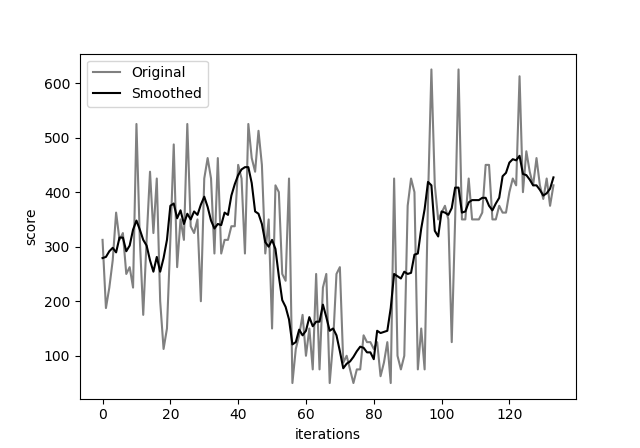
\includegraphics[width=\linewidth]{QbertNoiseComparison.png}
  \caption{Smoothing of training results.}
  \label{fig:noise_comp}
\end{figure}

During our testing we saw that in fact the introduction of novelty and weighting the optimization according to the results has a positive impact on the performance of the model, as can be seen in Figure \ref{fig:comp_res}. In this figure we can see the at around 60 iterations the model gets into a local optima and this is where our algorithm differs form the CanonicalES algorithm, In our algorithm the weight of the novelty score gets higher and therefore we can observe an improvement at around iteration 80 that ultimately leads to a far better result then the CanonicalES algorithm which stays relatively in the same score.

\begin{figure}[h!]
  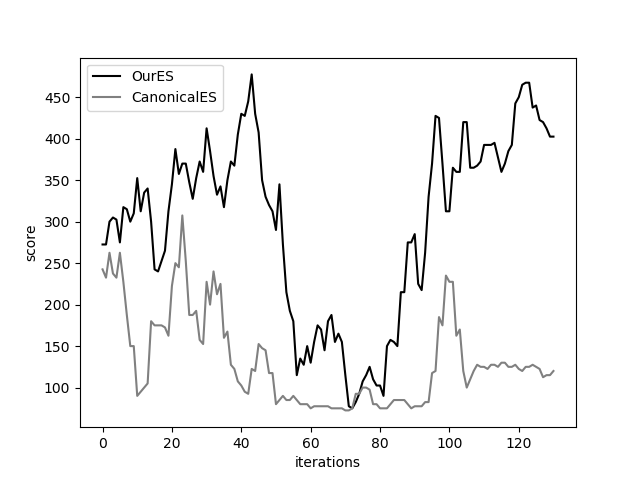
\includegraphics[width=\linewidth]{QbertComparison.png}
  \caption{Comparison of the same run with OurES and CanonicalES algorithms.}
  \label{fig:comp_res}
\end{figure}

\section{Conclusion}
To conclude it seems like the method we described to reduce the tendency of ES algorithms to plateau can indeed improve existing methods and lead to better results. Although we had limited resource to use we still found that the method improves the result. We believe that applying this method using enough resources could lead to far better results. We also suggest to further investigate the use of Auto-Encoders or Deep Compression to compute the novelty score which can be used to record far more behavior representations and thus improve the application of the novelty concept to this problem.

\bibliography{when_AI_Gets_Bored} 
\bibliographystyle{ieeetr}
\end{document}